\clearpage

\section{시험 실행}\label{sec:runners}

\subsection{실행 구조}

시험 실행부는 시험 입력을 실제 프로토콜 메시지로 조립하여 대상과 주고받는다.
대상과 역할(표~\ref{tab:roles})마다 전용 실행기가 있으며, 모든 실행기는 같은 방식으로 다음 세 가지를 기록한다.
이 기록이 그대로 판정의 입력이 된다.

\begin{itemize}
    \item \textbf{보낸 메시지}와 그 메시지에 적용된 변형 및 의도 태그
    \item \textbf{받은 응답} (수락, 프로토콜 오류, 무응답, 연결 끊김)
    \item \textbf{세션 상태의 흐름}: 단계마다 기록한 인증 여부, 진행 중인 트랜잭션, 세션 식별자 등의 스냅샷
\end{itemize}

실행기는 새로운 프로토콜이나 역할을 추가할 때 다른 부분을 고치지 않고 등록만으로 연결되도록 분리되어 있다.

\subsection{충전기 시험}\label{subsec:listener}

충전기 시험에서는 충전기가 먼저 접속해 와야 하므로, 퍼저는 \textbf{시험과 독립된 대기 상태}(리스너)를 가진다(그림~\ref{fig:listener}).
사용자가 리스너를 시작하면 퍼저는 관제 서버처럼 접속을 기다리고, 접속해 온 충전기를 인증 정보와 허용 목록으로 걸러 받아들인다.
충전기의 부팅·인증·충전 보고에는 정상적인 서버 응답을 돌려주어 세션이 정상적으로 진행되게 하며, 필요하면 이 응답 자체를 변형하여 ``잘못된 서버 응답''에 대한 충전기의 견고성도 시험할 수 있다.
사용자가 연결된 충전기 중 하나를 선택하면 시험을 시작할 수 있다.

\begin{figure}[H]
\centering
\begin{tikzpicture}[every node/.style={font=\footnotesize}]
  \node[box, minimum width=32mm] (l)    at (0,0)     {리스너 시작\\\scriptsize 관제 서버로 대기};
  \node[box, minimum width=32mm] (h)    at (4.6,0)   {충전기 접속\\\scriptsize 인증 · 허용 목록 확인};
  \node[box, minimum width=32mm] (b)    at (9.2,0)   {부팅 보고 수신\\\scriptsize 정상 응답으로 세션 진행};
  \node[box, minimum width=32mm] (hc)   at (0,-1.9)  {상태 확인\\\scriptsize 매 단계 직전};
  \node[box, minimum width=32mm] (c)    at (4.6,-1.9){시험 시작};
  \node[box, minimum width=32mm] (s)    at (9.2,-1.9){시험 대상 충전기 선택};
  \node[hot, minimum width=32mm] (step) at (0,-3.8)  {변형 명령 전송\\\scriptsize 응답 관측};
  \node[ext, minimum width=32mm] (rs)   at (4.6,-3.8){세션 재시작\\\scriptsize 충전기 재접속 대기};
  \node[ext, minimum width=32mm, draw=ksred] (dead) at (9.2,-3.8) {충전기 응답 불능 판정\\\scriptsize 시험 중단};
  \draw[arr] (l) -- (h);
  \draw[arr] (h) -- (b);
  \draw[arr] (b) -- (s);
  \draw[arr] (s) -- (c);
  \draw[arr] (c) -- (hc);
  \draw[arr] (hc) -- node[lbl, left]{정상} (step);
  \draw[arr] (hc.south east) -- node[lbl, fill=white, inner sep=1pt]{이상} (rs.north west);
  \draw[arr] (rs) -- node[lbl, fill=white, inner sep=1pt]{복구} (step);
  \draw[arr] (rs) -- node[lbl, above]{반복 실패} (dead);
  \draw[arr] (step.west) to[out=150, in=210] node[lbl, left]{다음 단계} (hc.west);
  \draw[arr, dashed] (h.north) to[out=150, in=30] node[lbl, above]{허용되지 않은 접속은 거부} (l.north);
\end{tikzpicture}
\caption{충전기 시험의 수명주기}
\label{fig:listener}
\end{figure}

그림~\ref{fig:ui-connect}는 웹 화면에서 이 과정을 진행하는 모습이다.
오른쪽 패널에서 프로토콜과 대상을 충전기로 고르면 \textbf{충전기가 접속할 주소}가 표시되고, 충전기가 이 주소로 접속하면 왼쪽 퍼저 블록의 \textbf{연결됨} 목록에 나타난다.
목록에서 충전기를 선택하면 시험을 시작할 수 있다. 예시는 실제 충전기 대신 모의 충전기(CP\_DEMO\_01)를 접속시킨 화면이다.

\begin{figure}[H]
    \centering
    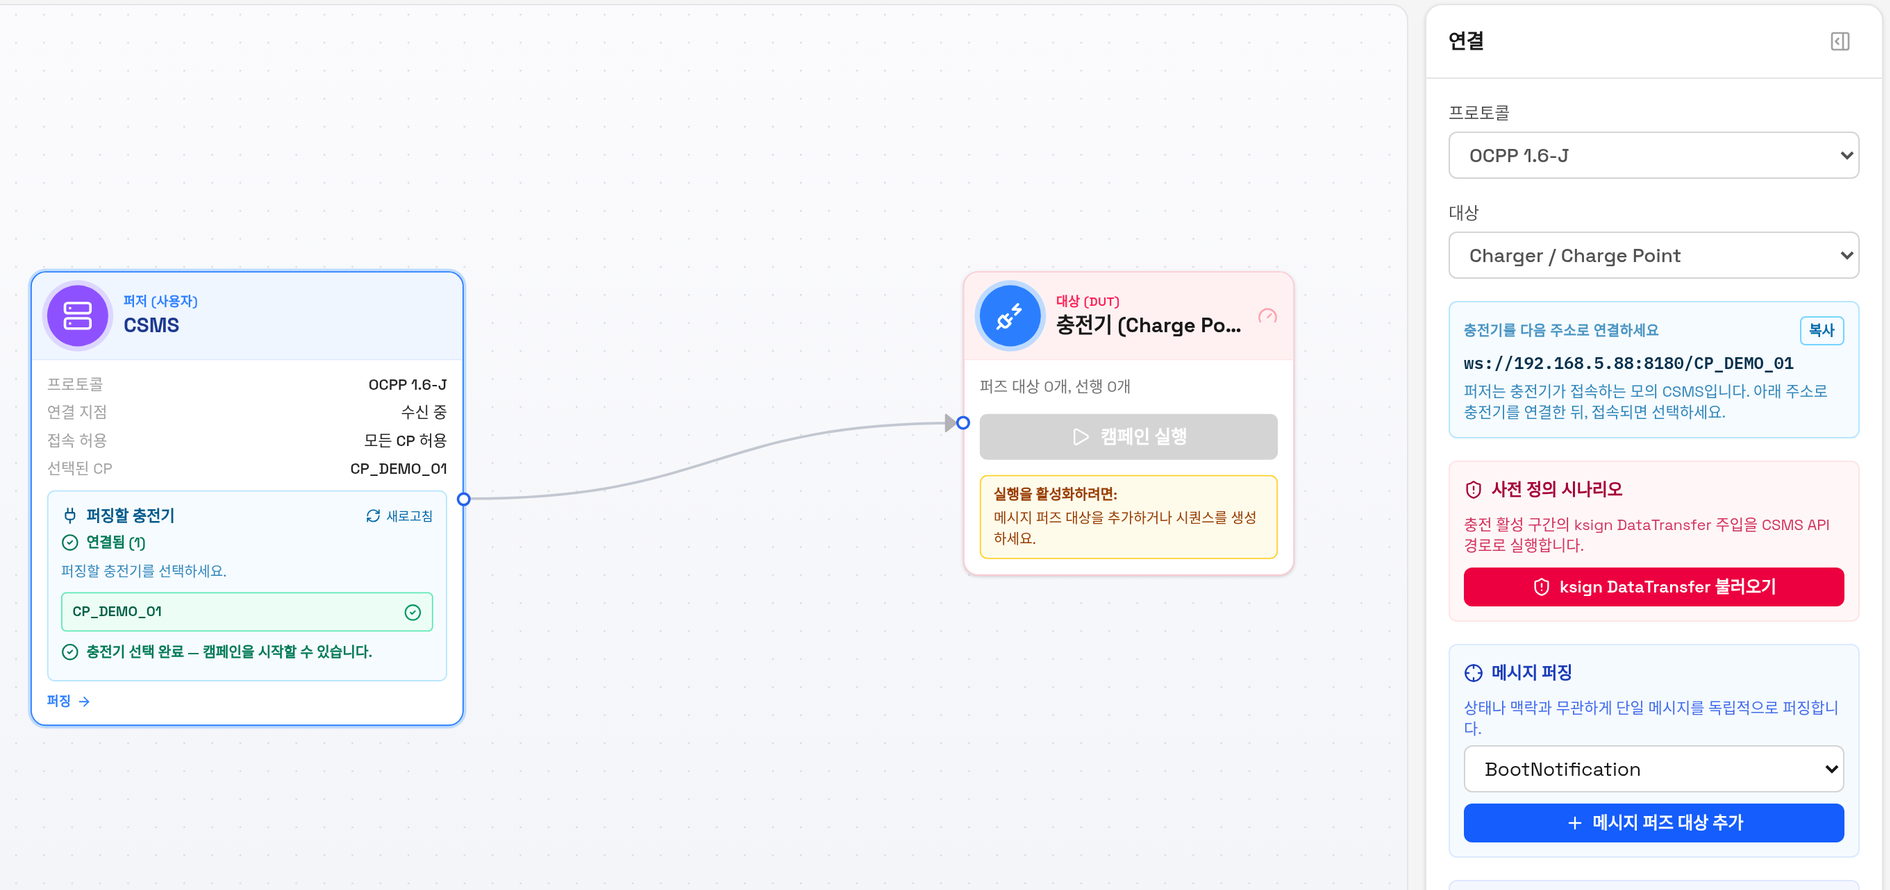
\includegraphics[width=\textwidth]{screenshots/ui01_connect_c.png}
    \caption{웹 화면: 충전기 접속 대기와 시험 대상 선택}
    \label{fig:ui-connect}
\end{figure}

\paragraph{상태 확인과 자동 복구.}
퍼징은 대상을 일부러 불안정하게 만드는 작업이므로, 한 번의 크래시가 이후 모든 시험을 의미 없는 타임아웃으로 만들 위험이 있다.
퍼저는 매 단계 직전에 연결이 살아 있는지 가벼운 신호와 무해한 조회 명령으로 확인하고, 이상이 있으면 충전기의 재접속을 기다려 세션을 복구한다.
복구가 반복해서 실패하면 충전기를 응답 불능으로 판정하고 남은 시험을 중단한다.
이렇게 하면 크래시 자체는 명확한 근거로 남고, 이후 결과가 오염되지 않는다.

\subsection{관제 서버 및 중간자 시험}

관제 서버 시험에서는 퍼저가 충전기로 동작하여 서버에 접속하고, 부팅·인증·충전 시작·계량·충전 종료 보고를 변형하여 보낸다.
서버의 응답에 따라 인증 여부와 트랜잭션 번호 같은 상태를 추적하며, 앞선 응답에서 받은 값(예: 트랜잭션 번호)을 다음 메시지에 이어 쓰는 방식으로 실제 충전 흐름을 재현한다.
로컬 시험 환경에서는 오픈소스 관제 서버(SteVe)를 대상으로 사용한다.

중간자 시험에서는 퍼저가 충전기와 관제 서버 사이에 들어가 양방향 메시지를 중계하면서 선택적으로 변형한다.

\subsection{ISO 15118 시험}

ISO 15118 시험에서는 퍼저가 차량 측 통신 제어기로 동작하여 충전기 측 제어기와 충전 협상을 진행한다.
메시지는 EXI(Efficient XML Interchange)로 압축 인코딩된 뒤 V2GTP 전송 프레임에 담겨 전달된다(그림~\ref{fig:v2gtp}).
퍼저는 메시지 내용뿐 아니라 프레임 헤더(버전, 페이로드 유형, 길이)도 변형 대상으로 삼을 수 있다.

\begin{figure}[H]
\centering
\begin{tikzpicture}[every node/.style={font=\scriptsize}]
  \def\h{7mm}
  \draw[ksblue, fill=kslight] (0,0) rectangle (16mm,\h) node[midway]{버전};
  \draw[ksblue, fill=kslight] (16mm,0) rectangle (32mm,\h) node[midway]{역버전};
  \draw[ksblue, fill=kslight] (32mm,0) rectangle (60mm,\h) node[midway]{페이로드 유형};
  \draw[ksblue, fill=kslight] (60mm,0) rectangle (100mm,\h) node[midway]{페이로드 길이};
  \draw[ksred, fill=white] (100mm,0) rectangle (145mm,\h) node[midway]{EXI 인코딩된 메시지};
  \node[lbl, below=1mm] at (50mm,0) {V2GTP 헤더 (8바이트)};
  \node[lbl, below=1mm] at (122mm,0) {충전 협상 메시지 본문};
\end{tikzpicture}
\caption{ISO 15118 메시지 전송 프레임}
\label{fig:v2gtp}
\end{figure}

EXI 인코딩은 교체 가능한 구성 요소로 분리되어 있어, 시험용 간이 인코더와 실제 EXI 구현을 상황에 맞게 선택할 수 있다.
어떤 인코더로 시험했는지는 결과의 근거에 함께 기록되어 판정의 신뢰도를 해석하는 데 쓰인다.

\subsection{관제 서버 경유 공격 시나리오}

퍼저가 충전기와 직접 연결하지 않고, 충전기가 접속해 있는 관제 서버(SteVe)의 시험용 인터페이스를 통해 충전기로 메시지를 주입하는 경로도 제공한다.
이 시나리오는 충전기 연결 확인, 인증 태그 등록, 정상 관제 명령, 충전 활성 확인, 공격 메시지 주입 순으로 진행되며 2단계 캠페인 방식을 따른다.
공격 후에는 충전기가 연결을 유지하는지, 공격 메시지를 거부했는지, 응답했는지를 보고 결과를 판정한다.
같은 공격은 \ref{subsec:listener}절의 직접 연결 방식으로도 실행할 수 있으며, 두 경로는 동일한 공격 메시지를 사용한다.
